\section{Planning: The DMP}
{
    \setbeamertemplate{background canvas}{
        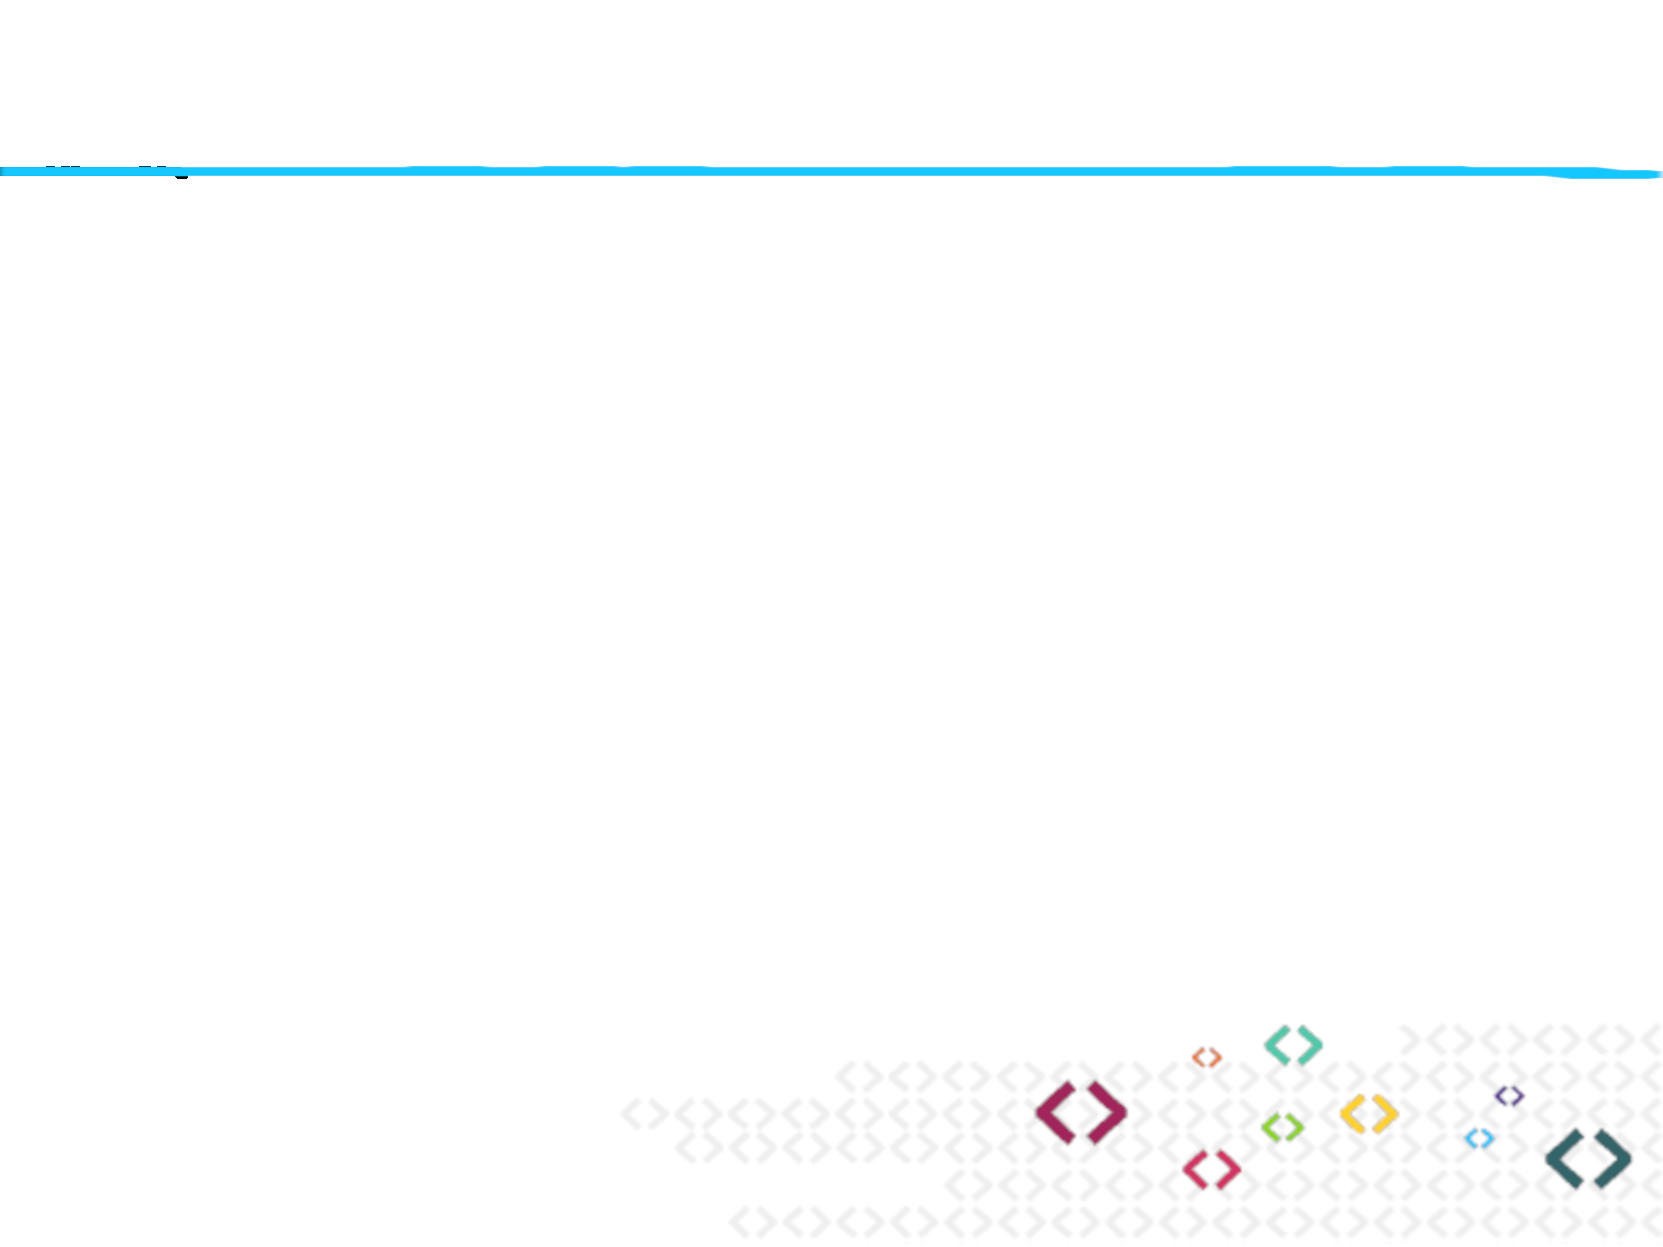
\includegraphics[width=\paperwidth,height=\paperheight]{figs/background_white.png}
    }
    \begin{frame}[plain]{Day 1 - Part 2: The Planning Phase}{10:50 - 11:35}
        \begin{block}{Module 2 Goal}
            To master the \textbf{Data Management Plan (DMP)} as our primary tool for \textit{planning} a FAIR publication, using the \textbf{RDMO} tool.
        \end{block}
        \begin{center}
            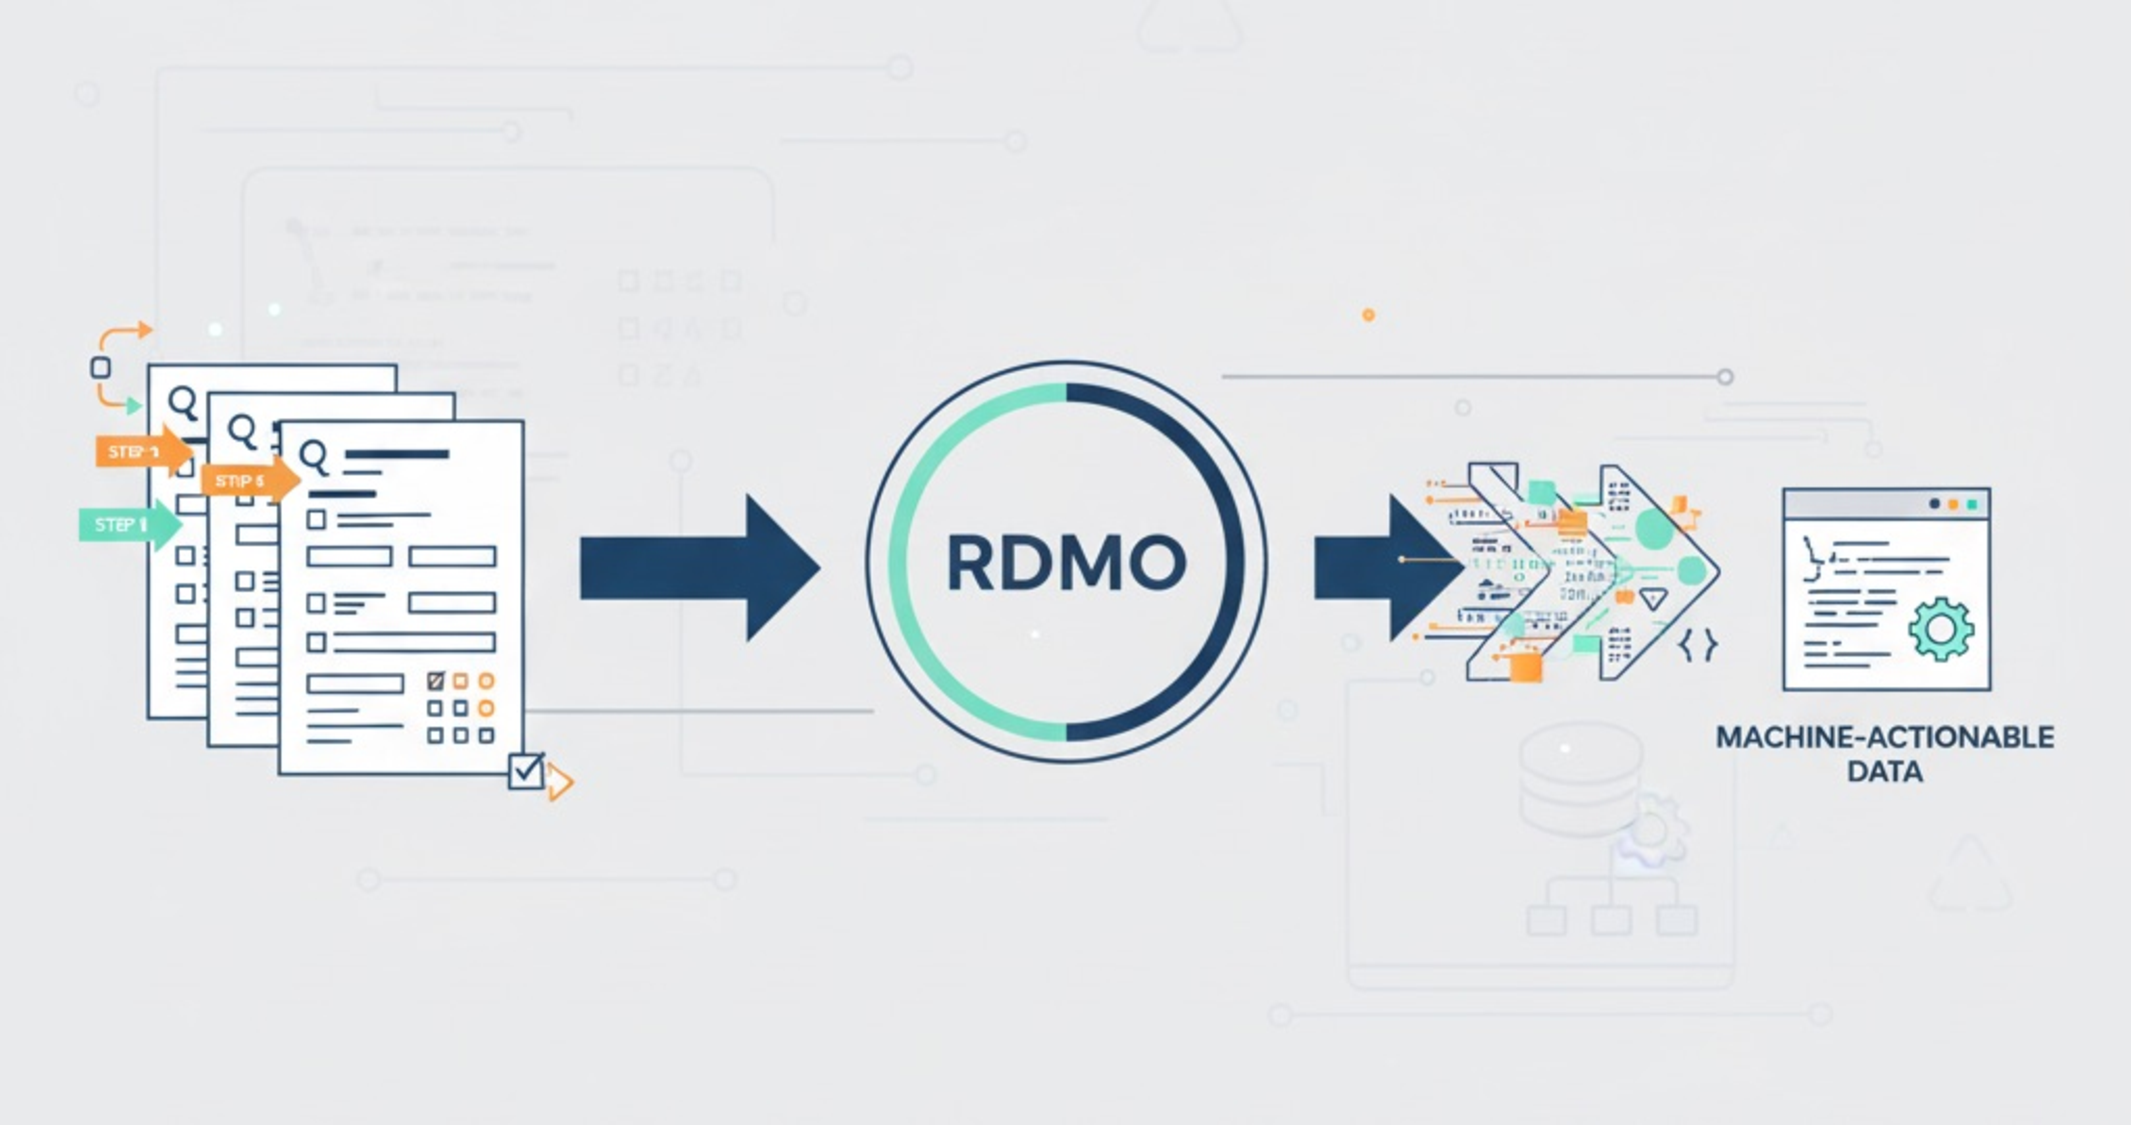
\includegraphics[width=0.32\textwidth]{figs/fig_d1p2/d1p2_01-blueprint}
            \captionof{figure}{A DMP is the blueprint for your research data.}
        \end{center}
    \end{frame}
}

\begin{frame}{Learning Objectives (2.1)}
    \begin{itemize}
        \item \textbf{Define} the four core elements of the FAIR acronym (Refresher).
        \item \textbf{Identify} the specific RDMO question categories (e.g. \emph{Metadata}, \emph{Documentation}, \emph{Long-term Preservation}) that correspond directly to each of the four FAIR principles.
    \end{itemize}
\end{frame}

\begin{frame}{Theory: What is RDMO?}{Module 2.1: Identify}
    \begin{columns}
        \column{.74\textwidth}
        The \textbf{Research Data Management Organiser (RDMO)} is a tool to support the systematic planning, implementation, and management of research data.
        \pause
        \begin{itemize}
            \item It's a "smart questionnaire."
            \item It guides you through the questions funders (like DFG) want answered.
            \item It generates a human-readable and machine-readable DMP.
            \item It is hosted by KIT!
        \end{itemize}
        
        \column{.36\textwidth}
        \begin{center}
            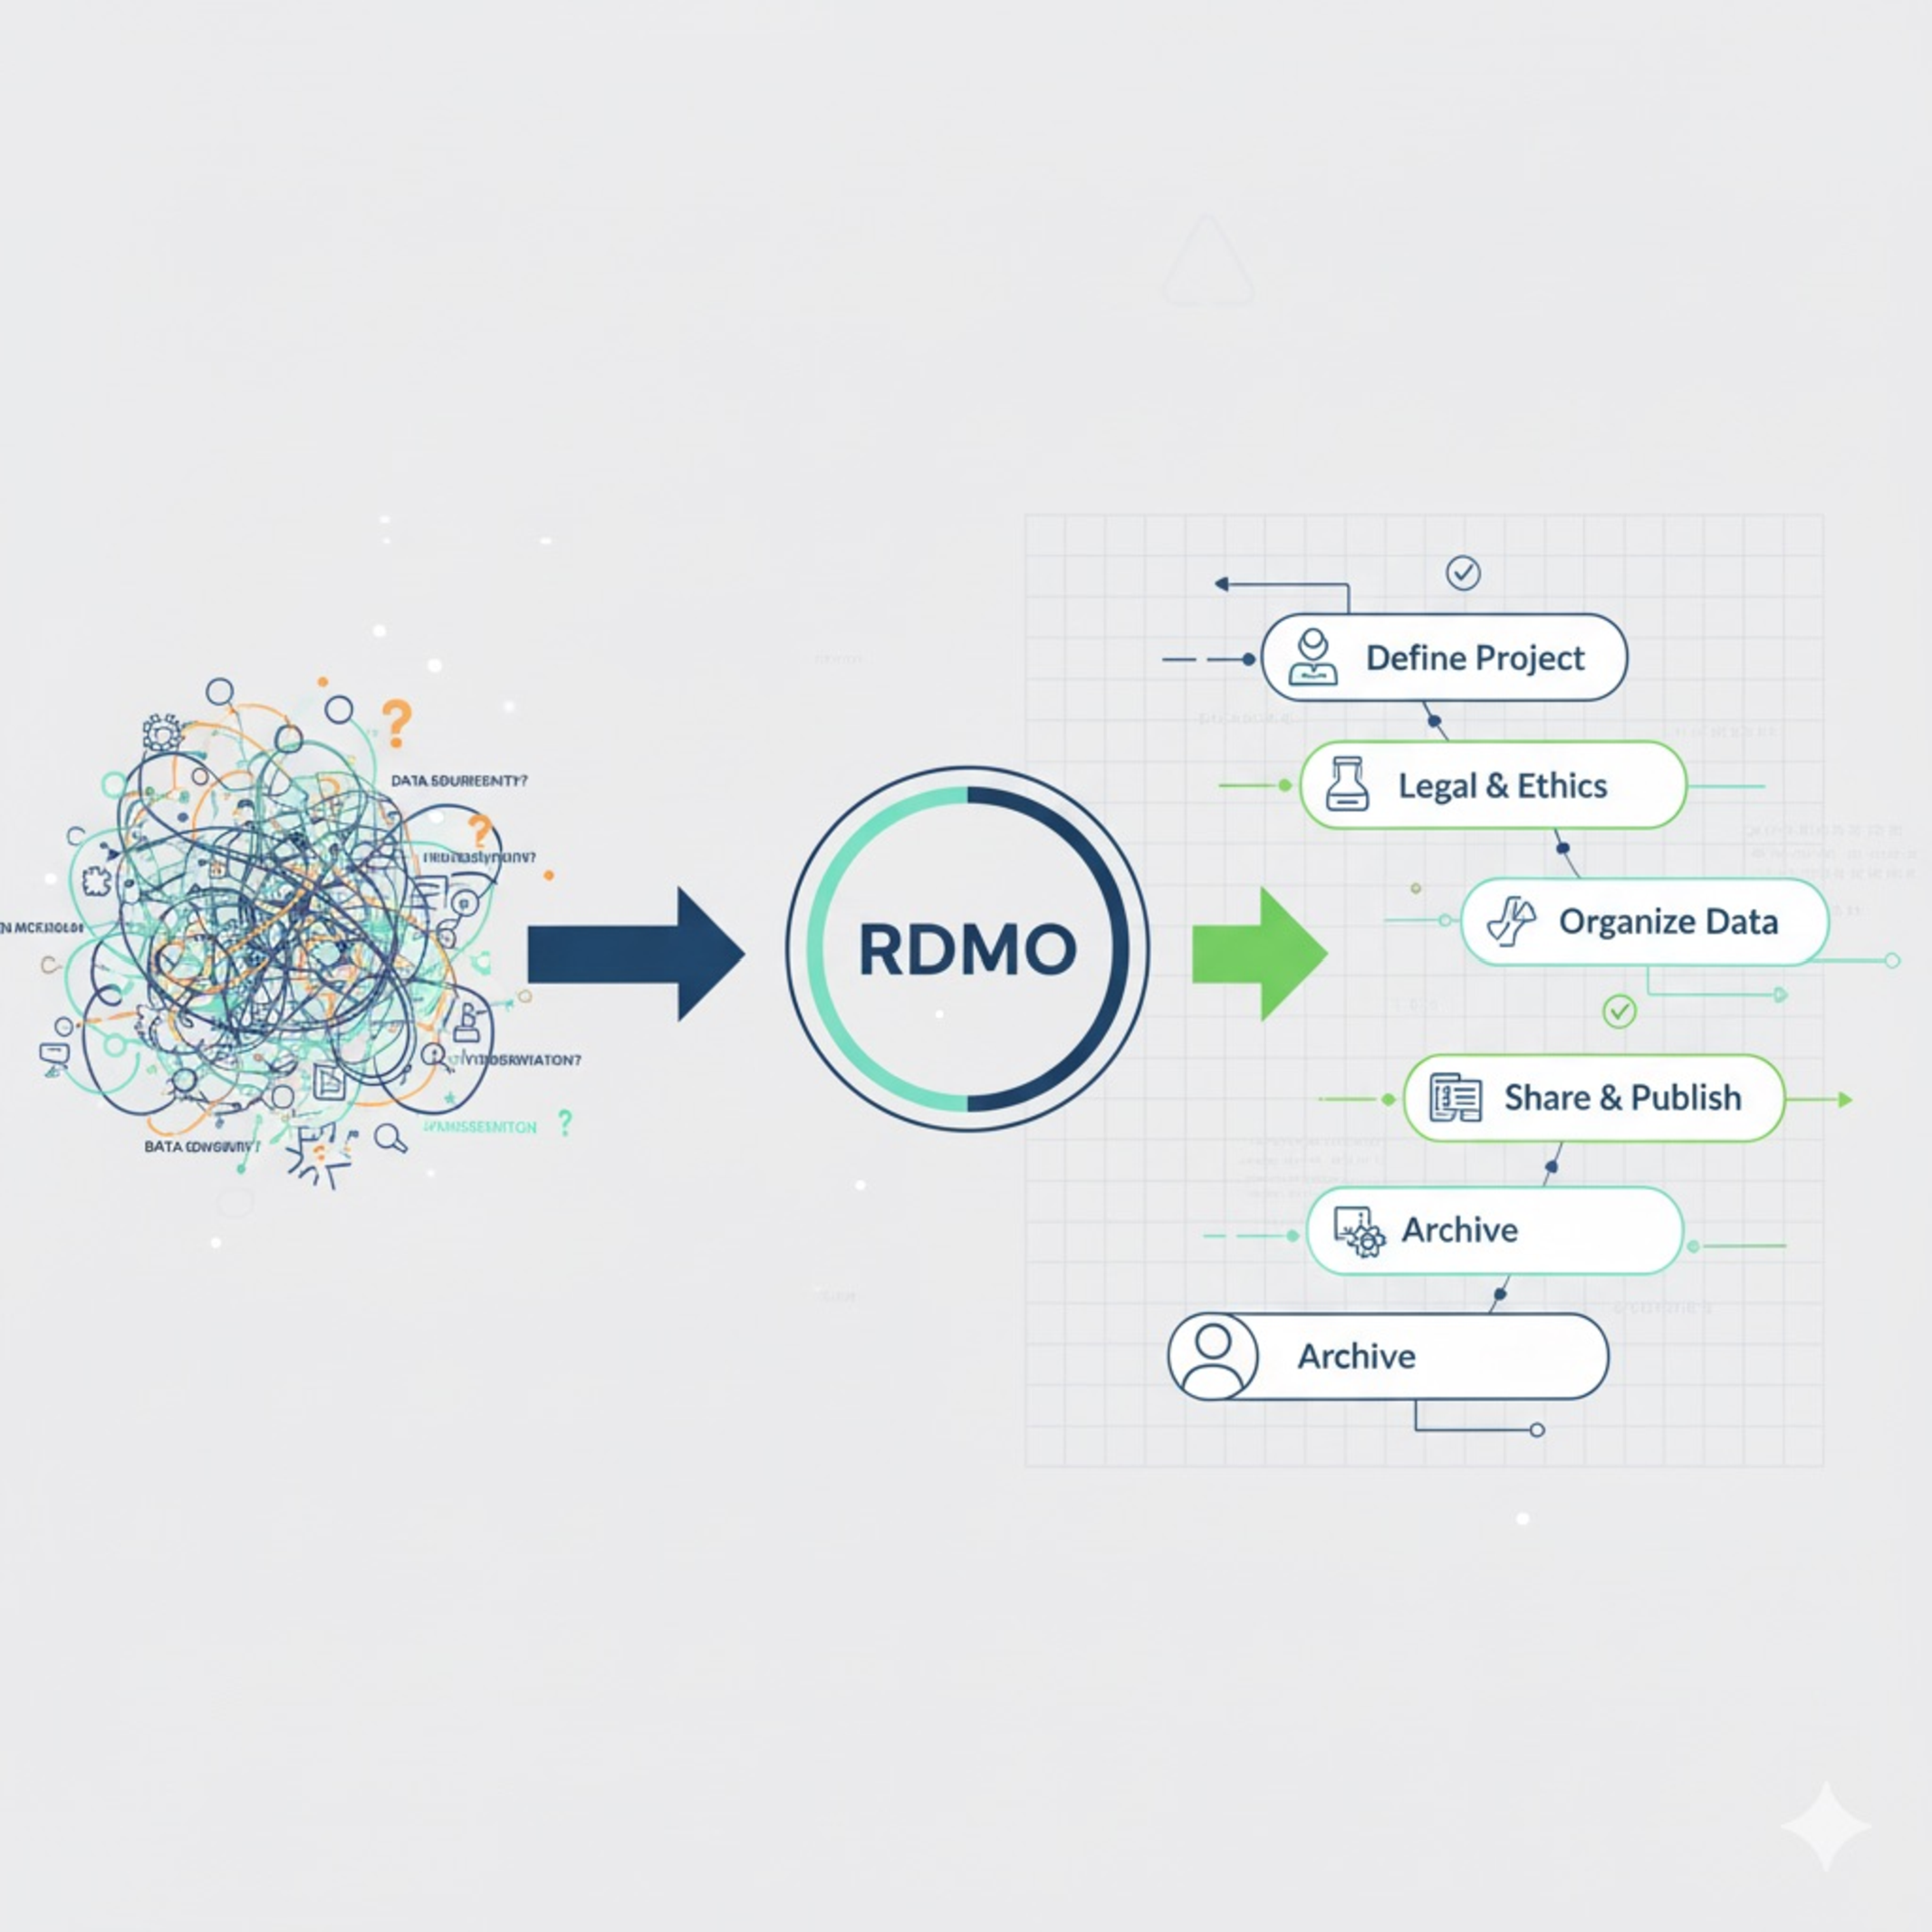
\includegraphics[width=.8\textwidth]{figs/fig_d1p2/d1p2_02-path}
        \end{center}
        \captionof{figure}{RDMO turns chaos into a structure}
    \end{columns}
\end{frame}

\begin{frame}{Concept: Mapping FAIR to RDMO}{Module 2.1: Identify}
    RDMO is structured around the RDM lifecycle, which maps directly to FAIR.
    
    \begin{itemize}
        \item \textbf{To be 'Findable' (F)...}
        \pause
        \item \textit{RDMO asks about:} "Project \& Data," "PIDs," "Repository."
        \pause
        \item \textbf{To be 'Accessible' (A)...}
        \pause
        \item \textit{RDMO asks about:} "Access \& Re-use," "Legal \& Ethical."
        \pause
        \item \textbf{To be 'Interoperable' (I)...}
        \pause
        \item \textit{RDMO asks about:} "Metadata," "Vocabularies," "Formats."
        \pause
        \item \textbf{To be 'Reusable' (R)...}
        \pause
        \item \textit{RDMO asks about:} "Documentation," "Licensing," "Quality."
    \end{itemize}
\end{frame}

\begin{frame}{Interactive: RDMO Treasure Hunt}{Module 2.1: Practice}
    \begin{block}{Activity: Log into RDMO (10 min)}
        \textbf{Task:} Log into the KIT RDMO instance. Create a new dummy project (use the "DFG" template).\\
        \pause
        \textbf{Challenge:} \textbf{Identify} the \textit{exact question} in RDMO that asks...
        \begin{itemize}
            \item How you will license your data ('R')?
            \item What metadata standard will you use ('I')?
            \item If your data will have a PID ('F')?
        \end{itemize}
        \pause
        \textbf{Goal:} \textbf{Identify} how RDMO is structured around FAIR. \\
        \textbf{URL:} \href{https://rdmorganiser.github.io}{https://rdmorganiser.github.io} \& \href{https://github.com/rdmorganiser/rdmo-docker-compose}{rdmo-docker-compose}
    \end{block}
\end{frame}

\begin{frame}{Learning Objectives (2.2)}
    \begin{itemize}
        \item \textbf{Explain} \emph{why} addressing the 'F' (Findable) principle is critical during the \textit{planning} phase.
        \item \textbf{Explain} how the structured output format of the RDMO tool supports the \textbf{Interoperability} ('I') of the DMP itself.
    \end{itemize}
\end{frame}

\begin{frame}{Theory: Why 'Findable' is a Planning Task}{Module 2.2: Explain}
    \begin{columns}
        \column{.64\textwidth}
        You can't make data "findable" \textit{after} the project is over. It's too late.
        \pause
        \begin{itemize}
            \item \textbf{Planning for 'F'} means deciding \textit{before you collect data}:
            \pause
            \item \textbf{Where} will it be published? (e.g., KITOpen)
            \item \textbf{What} is the PID strategy? (e.g., We will get a DOI)
            \item \textbf{How} will it be described? (e.g., We will use Dublin Core)
        \end{itemize}
        \pause
        If you don't plan for this, you end up with data on a hard drive that nobody (not even you) can find.
        
        \column{.36\textwidth}
        \begin{center}
            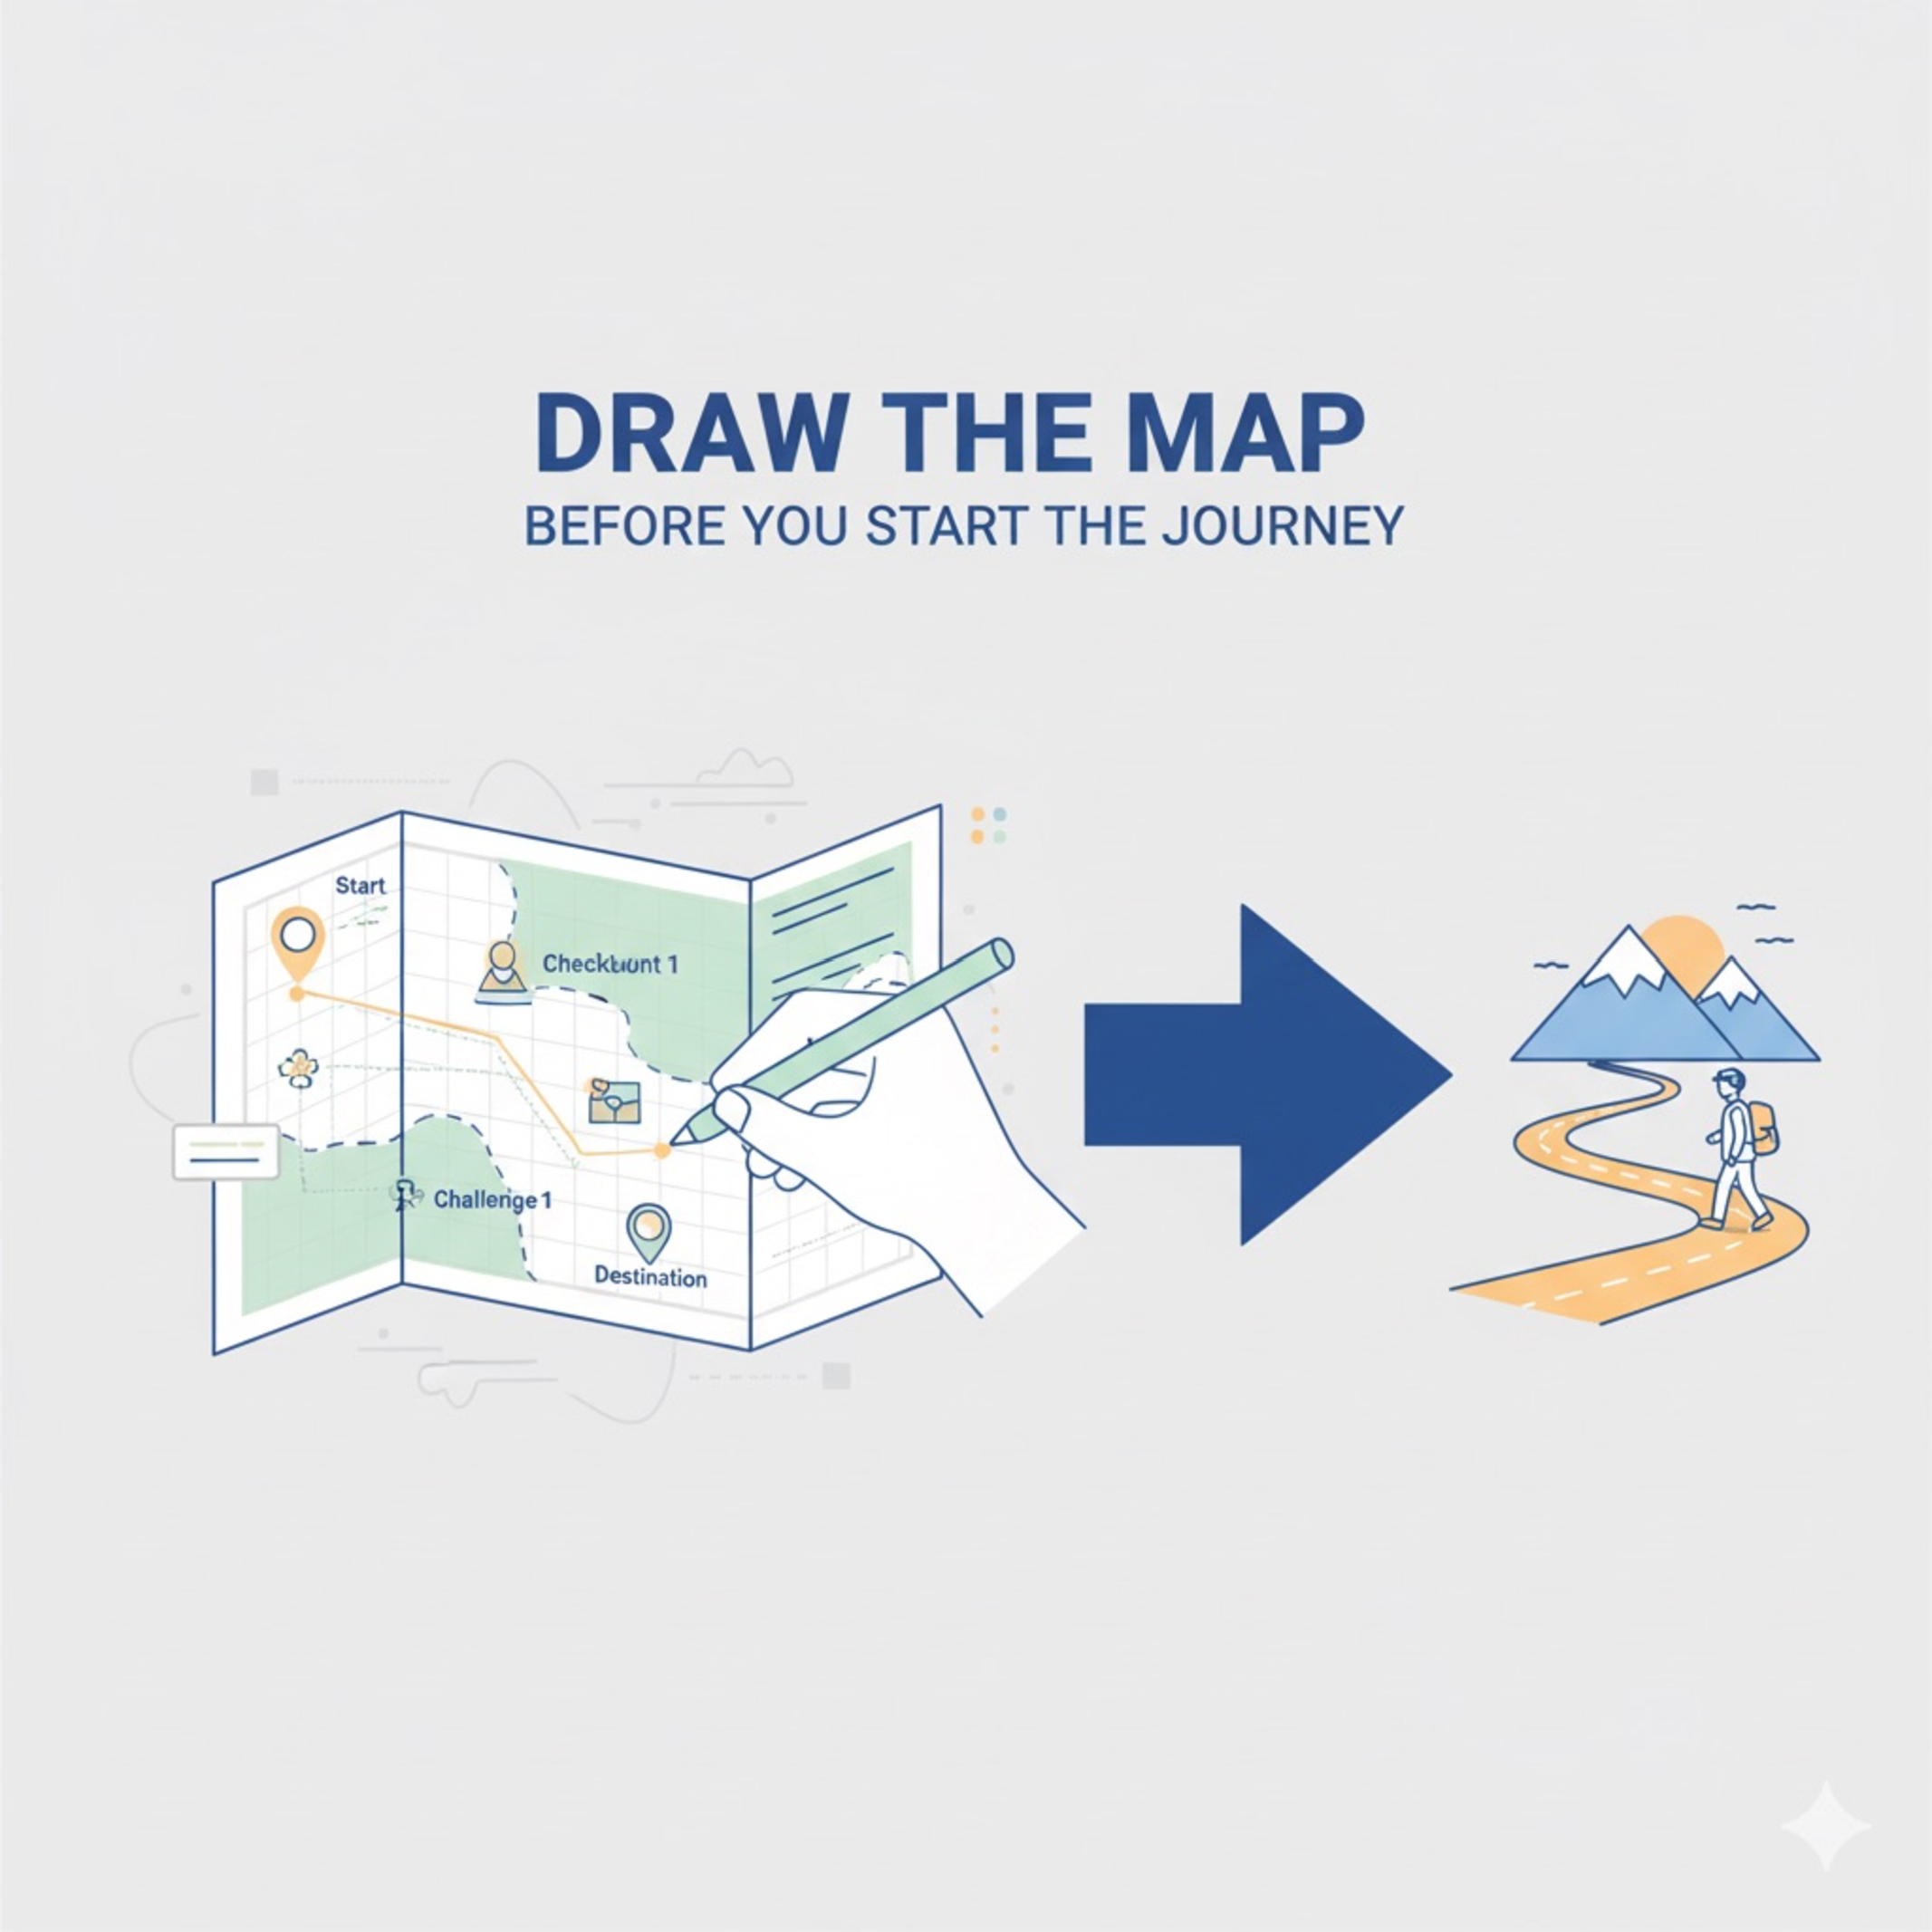
\includegraphics[width=.64\textwidth]{figs/fig_d1p2/d1p2_03-map}
       
        \end{center}
        \captionof{figure}{Draw the map \textit{before} you start the journey}
    \end{columns}
\end{frame}

\begin{frame}{Theory: RDMO for Interoperability ('I')}{Module 2.2: Explain}
    The DMP from RDMO isn't just a text document. It's a structured, machine-readable database entry.
    
    \begin{block}{The 'I' of the DMP Itself}
        You can \textbf{export} your DMP from RDMO in formats like:
        \begin{itemize}
            \item XML
            \item JSON
            \item etc. (RDMO-Instance dependant)
            \pause
            \item This means your \emph{plan} is now interoperable. It can be automatically read by funders (DFG), repositories (KITOpen), or other project management tools.
            \pause
            \item This is "FAIR for your DMP."
        \end{itemize}
    \end{block}
\end{frame}

\begin{frame}{Interactive: The "Why" of Planning}{Module 2.2: Practice}
    \begin{block}{Group Discussion (10 min)}
        \textbf{Scenario:} A researcher says, "I'm too busy doing research to write a DMP. I'll document my data when I'm finished."
        \pause
        \textbf{Task:}
        \begin{itemize}
            \item \textbf{Explain} to this researcher why this is a bad idea, using the 'F' (Findable) principle.
            \pause
            \item \textbf{Explain} how spending 2 hours on RDMO now will save them 20 hours later.
        \end{itemize}
    \end{block}
\end{frame}

\begin{frame}{Learning Objectives (2.3)}
    \begin{itemize}
        \item \textbf{Determine} the appropriate persistent identifier (e.g. DOI, Handle, ARK) to be used for the planned dataset.
        \item \textbf{Determine} and input the required \textbf{Persistent Identifier (PID) strategy} into the RDMO questionnaire.
    \end{itemize}
\end{frame}

\begin{frame}{Theory: The PID Landscape}{Module 2.3: Determine}
    A Persistent Identifier (PID) is a long-lasting reference to a digital object.
    
    \begin{columns}
        \column{.5\textwidth}
        \begin{block}{Common PIDs}
            \begin{itemize}
                \item \textbf{DOI (Digital Object Identifier):} Most common for publications and datasets. Excellent for citation.
                \item \textbf{Handle:} The system that DOIs are built on.
                \item \textbf{ARK (Archival Resource Key):} Common in libraries and archives.
                \item \textbf{ORCID:} A PID for \emph{people}.
            \end{itemize}
        \end{block}
        
        \column{.5\textwidth}
        \begin{block}{Your Strategy}
            For 99\% of researchers at Helmholtz, the strategy is simple:
            \pause
            "I will deposit my data in a repository (like KITOpen) that will mint a \textbf{DOI} for me."
            \pause
            Your job is not to \emph{create} the DOI, but to \emph{plan} on getting one.
        \end{block}
    \end{columns}
\end{frame}

\begin{frame}{Concept: Why Not Just Use a URL?}{Module 2.3: Determine}
    %% \begin{center}
    %%     \includegraphics[width=0.6\textwidth]{example-image-b}
    %%     \captionof{figure}{A URL is an address. A PID is a name.}
    %% \end{center}
    
    \begin{itemize}
        \item A standard URL (`http://my-lab.kit.edu/data.zip`) is \textbf{not persistent}.
        \item What happens when the website is redesigned? The server is changed? The researcher leaves?
        \item $\rightarrow$ \textbf{Link Rot!} The link is broken. The data is lost.
        \pause
        \item A \textbf{PID} (like a DOI) points to a \textit{resolver} (e.g., doi.org), which then redirects to the \textit{current} URL. If the URL changes (e.g., KITOpen moves servers), the repository updates the resolver. The DOI never changes.
    \end{itemize}
\end{frame}

\begin{frame}{Interactive: Your PID Strategy}{Module 2.3: Practice}
    \begin{block}{Workshop: Fill in the DMP (10 min)}
        \textbf{Task:} Go back to your draft RDMO plan.
        \pause
        \begin{enumerate}
            \item Find the section on "PIDs" or "Identifiers."
            \item \textbf{Determine} your PID strategy.
            \item \textbf{Input} your strategy.
        \end{enumerate}
        \pause
        \textbf{Example Answer:} "We will publish the final dataset in KITOpen to obtain a DOI. We will use this DOI in all publications that cite the data. Internal datasets will be identified using the HMC naming convention."
    \end{block}
\end{frame}

\begin{frame}{Learning Objectives (2.4)}
    \begin{itemize}
        \item \textbf{Distinguish} between an \emph{open} license (CC-BY) and a \emph{restrictive} license (CC-BY-NC-ND).
        \item \textbf{Justify} the selection of a specific \textbf{data access restriction model} (e.g., under embargo) in RDMO.
    \end{itemize}
\end{frame}

\begin{frame}{Theory: The License Spectrum}{Module 2.4: Distinguish}
    A license is the legal tool that makes data \textbf{Reusable ('R')}.
    
    \begin{block}{Creative Commons (CC) Licenses \href{https://creativecommons.org/share-your-work/cclicenses/}{$\therefore$}}
        \begin{itemize}
            \item \textbf{CC0 (Public Domain):} No rights reserved. The best for data!
            \pause
            \item \textbf{CC-BY (Attribution):} Anyone can use it, as long as they cite you. \textbf{(Recommended)}
            \pause
            \item \textbf{CC-BY-SA (ShareAlike):} They must also share their new work under CC-BY-SA.
            \pause
            \item \textbf{CC-BY-NC (Non-Commercial):} Cannot be used for commercial purposes. (Restricts 'R'!)
            \pause
            \item \textbf{CC-BY-ND (No-Derivatives):} Cannot be changed. (e.g., can't combine it with other data. Kills 'R'!)
        \end{itemize}
    \end{block}
\end{frame}

\begin{frame}{Theory: Access Model vs. License}{Module 2.4: Justify}
    These are two different things!
    
    \begin{itemize}
        \item \textbf{License:} What can people \emph{legally} do with your data \textit{if} they have it? (e.g., CC-BY)
        \pause
        \item \textbf{Access Model:} \textit{Who} can get the data in the first place?
        \begin{itemize}
            \item \textbf{Open Access:} Everyone.
            \item \textbf{Embargoed:} Open, but only \textit{after} a certain date (e.g., 1 year after publication).
            \item \textbf{Restricted:} Only specific people (e.g., collaborators) can access it after application.
            \item \textbf{Closed:} No one can access it.
        \end{itemize}
    \end{itemize}
    \pause
    \begin{block}{Key Idea}
        You can have an \textbf{Open License} (CC-BY) on \textbf{Restricted Data}. This means "If I approve your access, you are then free to use this data as long as you cite me."
    \end{block}
\end{frame}

\begin{frame}{Interactive: Debate - Access vs. Restriction}{Module 2.4: Practice}
    \begin{block}{Group Debate (15 min)}
        \textbf{Scenario:} Your data is publicly funded (DFG) but contains potentially patentable information.
        \pause
        \begin{columns}
            \column{.5\textwidth}
            \textbf{Group 1: Argue for...}
            \begin{itemize}
                \item Open Access
                \item CC-BY License
            \end{itemize}
            (Hint: DFG requirements, fast science)
            
            \column{.5\textwidth}
            \textbf{Group 2: Argue for...}
            \begin{itemize}
                \item Embargoed Access
                \item Restrictive License
            \end{itemize}
            (Hint: KIT tech transfer, patents)
        \end{columns}
        \pause
        \textbf{Goal:} \textbf{Justify} your data access restriction model.
    \end{block}
\end{frame}

\begin{frame}{Learning Objectives (2.5)}
    \begin{itemize}
        \item \textbf{Justify} the selection of a discipline-specific metadata standard over a general standard.
        \item \textbf{Appraise} a draft DMP against the DFG "Checklist for Handling of Research Data."
    \end{itemize}
\end{frame}

% \begin{frame}{Theory: General vs. Domain Standards}
%     \frametitle{Module 2.5: Justify}
%     \begin{columns}
%         \column{.5\textwidth}
%         \begin{block}{General Standard (e.g., Dublin Core)}
%             \begin{itemize}
%                 \item \textbf{Fields:} Creator, Title, Date, Publisher...
%                 \item \textbf{Pro:} Simple, universal. Good for 'F' and 'A'.
%                 \item \textbf{Con:} Can't describe \emph{what the data is}.
%                 \item \textbf{Metaphor:} A general library card catalog.
%             \end{itemize}
%         \end{block}
%         
%         \column{.5\textwidth}
%         \begin{block}{Domain Standard (e.g., OME-XML)}
%             \begin{itemize}
%                 \item \textbf{Fields:} `MicroscopeModel`, `LensMagnification`, `\texttt{Exposure_Time}`...
%                 \item \textbf{Pro:} Richly descriptive. Essential for 'I' and 'R'.
%                 \item \textbf{Con:} Complex, only used by experts.
%                 \item \textbf{Metaphor:} A specialized medical chart.
%             \end{itemize}
%         \end{block}
%     \end{columns}
%     \pause
%     \textbf{Justification:} "We will use Dublin Core for general findability on KITOpen, but we will \emph{also} include a `\texttt{metadata_ome.xml}` file for domain-specific reusability."
% \end{frame}

\begin{frame}{Concept: The DFG Checklist}{Module 2.5: Appraise}
    %% \begin{center}
    %%     \includegraphics[width=0.4\textwidth]{example-image-c}
    %%     \captionof{figure}{The DFG Checklist is your evaluation rubric.}
    %% \end{center}
    
    The DFG provides a "Checklist for Handling of Research Data" in its proposals. This is the list the reviewers will use to \textbf{appraise} your plan.
    \pause
    \begin{block}{Key DFG Checklist Items}
        \begin{itemize}
            \item "What data will be collected?"
            \item "What metadata standards will be used?"
            \item "Who is responsible for the data?"
            \item "How will the data be archived for 10 years?"
            \item "What costs are associated with this?"
        \end{itemize}
    \end{block}
\end{frame}

\begin{frame}{Interactive: Peer Review Your DMP}{Module 2.5: Practice}
    \begin{block}{Peer Review (15 min)}
        \textbf{Task:} Swap your draft RDMO plan (or the link) with a partner.
        \pause
        \textbf{Review:} \textbf{Appraise} your partner's DMP using the DFG Checklist.
        \pause
        \begin{itemize}
            \item Can you find the answer to "What metadata standard will be used?"
            \item Is their plan for 'Reusability' (licenses, documentation) clear?
            \item Give one piece of constructive feedback.
        \end{itemize}
        \pause
        \textbf{Goal:} \textbf{Appraise} a draft DMP and help improve it.
    \end{block}
\end{frame}

\begin{frame}{Learning Objectives (2.6)}
    \begin{itemize}
        \item \textbf{Develop} a comprehensive DMP section for the 'A' (Accessible) principle.
        \item \textbf{Generate} a complete, funder-compliant DMP for a research proposal using the RDMO tool.
    \end{itemize}
\end{frame}

\begin{frame}{Theory: Sub-Principles of 'Accessible'}{Module 2.6: Develop}
    'Accessible' is more than just "it's on the web."
    
    \begin{itemize}
        \item \textbf{A1:} (Meta)data are retrievable by their identifier using a standardised communications protocol.
        \item \textit{Your DMP Entry:} "Data will be deposited in KITOpen, which provides retrieval via HTTP and assigns a DOI."
        \pause
        \item \textbf{A1.1:} The protocol is open, free, and universally implementable.
        \item \textit{Your DMP Entry:} "The chosen protocol is HTTP(S), which is open."
        \pause
        \item \textbf{A1.2:} The protocol allows for an authentication and authorisation procedure, where necessary.
        \item \textit{Your DMP Entry:} "%For open data, no authentication is needed. For restricted data, 
        KITOpen manages authorisation."
        \pause
        \item \textbf{A2:} Metadata are accessible, even when the data are no longer available.
        \item \textit{Your DMP Entry:} "The repository (KITOpen) guarantees metadata persistence even if the data is removed."
    \end{itemize}
\end{frame}

\begin{frame}{Interactive: Finalize Your DMP}{Module 2.6: Practice}
    \begin{block}{Workshop (20 min)}
        \textbf{Task:} Go back to your RDMO plan one last time.
        \pause
        \begin{enumerate}
            \item Review your answers for 'Access' (Module 2.4) and 'Metadata' (Module 2.5).
            \pause
            \item Ensure every question has a clear, concise, and specific answer. (e.g., change "a repository" to "KITOpen").
            \pause
            \item Click the "Export" button and look at the generated document.
        \end{enumerate}
        \pause
        \textbf{Goal:} \textbf{Generate} a complete, funder-compliant DMP.
    \end{block}
\end{frame}

\begin{frame}{Module 2: Summary}
    \begin{itemize}
        \item The \textbf{DMP} is the central \emph{planning} document for FAIR.
        \item \textbf{RDMO} is the tool that guides us through this plan.
        \item We must plan for \textbf{PIDs ('F')}, \textbf{Licenses ('R')}, \textbf{Access ('A')}, and \textbf{Standards ('I')} from Day 1.
        \item A good DMP is the \textbf{blueprint} for your research and the key to your funding proposal.
    \end{itemize}
    \vfill
    \begin{center}
        \textbf{End of Part 2}
    \end{center}
\end{frame}